\subsection{Intensität der TEM$_{00}$- und TEM$_{01}$-Mode}
\subsubsection{TEM$_{00}$-Mode}

Fitparameter sind die maximale Amplitude $I_0$, die Breite des Laser-Strahls $\omega$, nachdem dieser die Zerstreuungslinse durchlaufen hat, und die Verschiebung des Maximums entlang der x-Achse $x_0$. Die Messdaten sind in Tabelle \ref{tab:TEM_00} zu finden und der zugehörige Plot ist Abbildung \ref{fig:TEM_00}.

\begin{align}
	I_0 =  \SI{446+-23}{\nano\ampere}
\\
	\omega =  \SI{-11.2+-0.7}{\milli\meter}
 \\
	x_0 = \SI{3.55+-0.34}{\milli\meter}

\end{align}
	
 \begin{table}
    \centering
    \caption{Intensität der TEM$_{00}$-Mode entlang der x-Achse}
    \label{tab:TEM_00}
    \sisetup{parse-numbers=false}
    \begin{tabular}{
	S[table-format=3.1]
	S[table-format=3.2]
	}
	\toprule
<<<<<<< HEAD
	{x in \si{\milli\meter}}		& {I in \si{\nano\ampere}}		\\ 
||||||| merged common ancestors
	{I in \si{\nano\ampere}	}	& {x in \si{\milli\meter}}		\\ 
=======
	{I in \si{\nano\ampere}}		& {x in \si{\milli\meter}}		\\ 
>>>>>>> 8eaf5d34c5428e65c24c499d1f18f65cd0a182c8
	\midrule
    14.3  & 2.95   \\
13.0  & 4.95   \\
12.0  & 7.60   \\
11.0  & 11.92  \\
10.0  & 20.15  \\
9.0   & 34.00  \\
8.0   & 54.50  \\
7.0   & 89.00  \\
6.0   & 129.80 \\
5.0   & 173.90 \\
4.0   & 218.00 \\
3.0   & 285.00 \\
2.0   & 326.00 \\
1.0   & 314.00 \\
0.0   & 303.00 \\
-1.0  & 352.00 \\
-2.0  & 335.00 \\
-3.0  & 356.00 \\
-4.0  & 403.00 \\
-5.0  & 473.00 \\
-6.0  & 526.00 \\
-7.0  & 512.00 \\
-8.0  & 404.00 \\
-9.0  & 258.00 \\
-10.0 & 207.00 \\
-11.0 & 105.50 \\
-12.0 & 73.50  \\
-13.0 & 51.30  \\
-14.0 & 31.70  \\
-15.0 & 26.00  \\

    \bottomrule
    \end{tabular}
    \end{table}



\begin{figure}[h!]
	\centering
	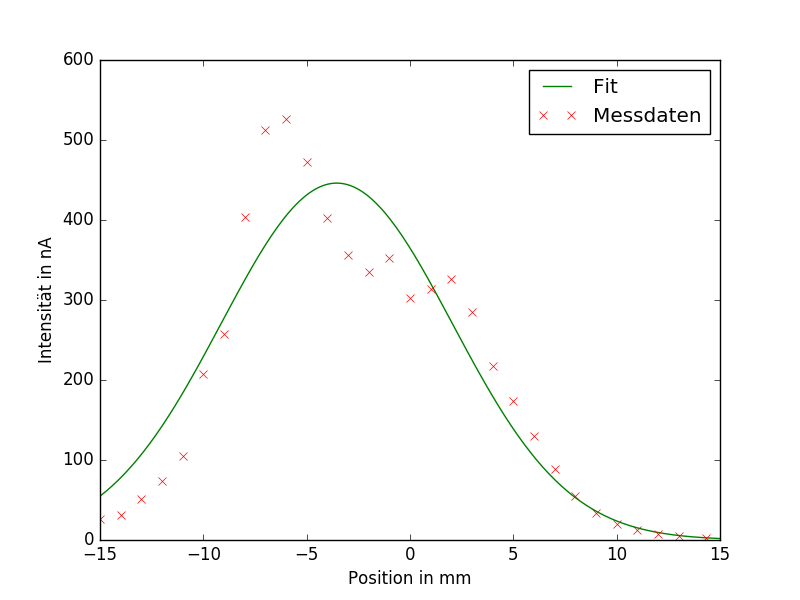
\includegraphics[width=.6\textwidth]{build/TEM_00.png}
	\caption{Intensität der TEM$_{00}$-Mode entlang der x-Achse gemessen}
	\label{fig:TEM_00}
\end{figure} 

blblblbl